\documentclass[a4paper,10pt]{article}
\usepackage[utf8]{inputenc}
\usepackage[T1]{fontenc}	
\usepackage[italian]{babel}

\usepackage{amsmath}
\usepackage{amsfonts}
\usepackage{amssymb}
\usepackage{graphicx}

\usepackage[left=2cm,right=2cm,top=2cm,bottom=2cm]{geometry}
\geometry{a4paper}

\usepackage{booktabs}
\usepackage{verbatim}
\usepackage{subfig}

\usepackage[cdot, thickqspace, squaren]{SIunits}
\usepackage{float}

% macro
\def\code#1{\texttt{#1}}

\title{Esperienza di Franck Hertz}
\author{Gruppo BL \\ Candido Alessandro, Luzio Andrea, Mazziotti Fabrizio}

\begin{document}

\maketitle

%\begin{abstract}
%Lo scopo di questa esperienza è di
%\end{abstract}

\section{Scopo e Strumentazione}
Lo scopo dell'esperienza è Misurare le caratteristiche statiche e dinamiche delle porte NOT contenute nell’integrato \code{SN74LS04} (HEX Inverter).

La strumentazione è quella solitamente presente sul banco di lavoro, e inoltre si è usato:
\begin{itemize}
	\item \code{IC SN74LS04};
	\begin{itemize}
		\item Trimmer da $2~$K e $100~$K;
	\end{itemize}
	\item Arduino Nano; 
	\begin{itemize}
		\item \code{IC SN74LS244} octal buffer/driver; 
		\item Trimmer da $10~$K;
	\end{itemize}
\end{itemize}

%\subsection{Errori sistematici}
%
%\begin{itemize}
%
% \item Oscilloscopio digitale Tektronix TDS 1012. \newline
% 		Lo strumento è affetto da erorre sistematico del 3 \% sulle scale di tensione utilizzate, e di 100 ppm sulle scale di tempo utilizzate.
% \item Tester digitale Konig KDM-350CTF. \newline con errore sistematico del 0.5 \% sulle scale di tensione, 0.8\% su tutte le scale di resistenza utilizzate. Per quanto riguarda l'errore sistematico relativo alle capacità è del 4\%.
%
%\end{itemize}

\section{Caratteristiche statiche}

\subsection{Misura delle tensioni di operazione}

\begin{figure}[H]
	\centering
	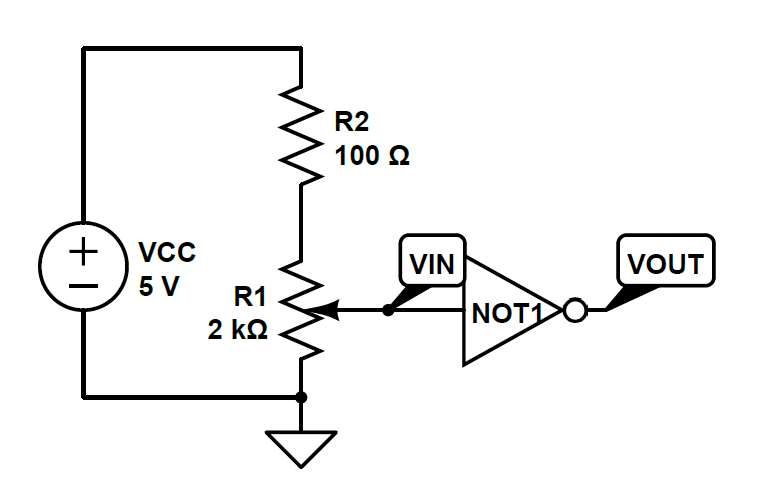
\includegraphics[width=0.7\textwidth]{../grafici/NOTin.png}
	\caption{}
	\label{fig:NOTin}
\end{figure}

\subsection{Misura delle correnti e del fanout}

\paragraph{Correnti in ingresso}

\paragraph{Correnti in uscita}

\begin{figure}[H]
	\centering
	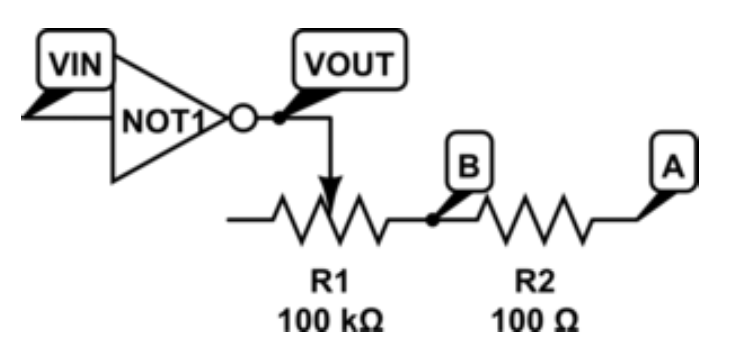
\includegraphics[width=0.5\textwidth]{../grafici/NOTout.png}
	\caption{}
	\label{fig:NOTout}
\end{figure}


\section{Montaggio di Arduino}

\section{Caratteristiche dinamiche}

\subsection{Misura dei tempi di propagazione}

\subsection{Misura del tempo di salita}

\end{document}